\section{Air Quality}
\subsection{Air pollution and its health effects}
Air pollution can be defined as a group of chemicals present in the atmosphere that are harmful to humans, animals or vegetation. It is mainly caused by human activities, such as transport, industry, or agriculture. However, it can also be influenced by other natural sources. Understanding air pollution is important because many health consequences are the result off high pollution levels. 
\begin{figure}[h]
  \centering
  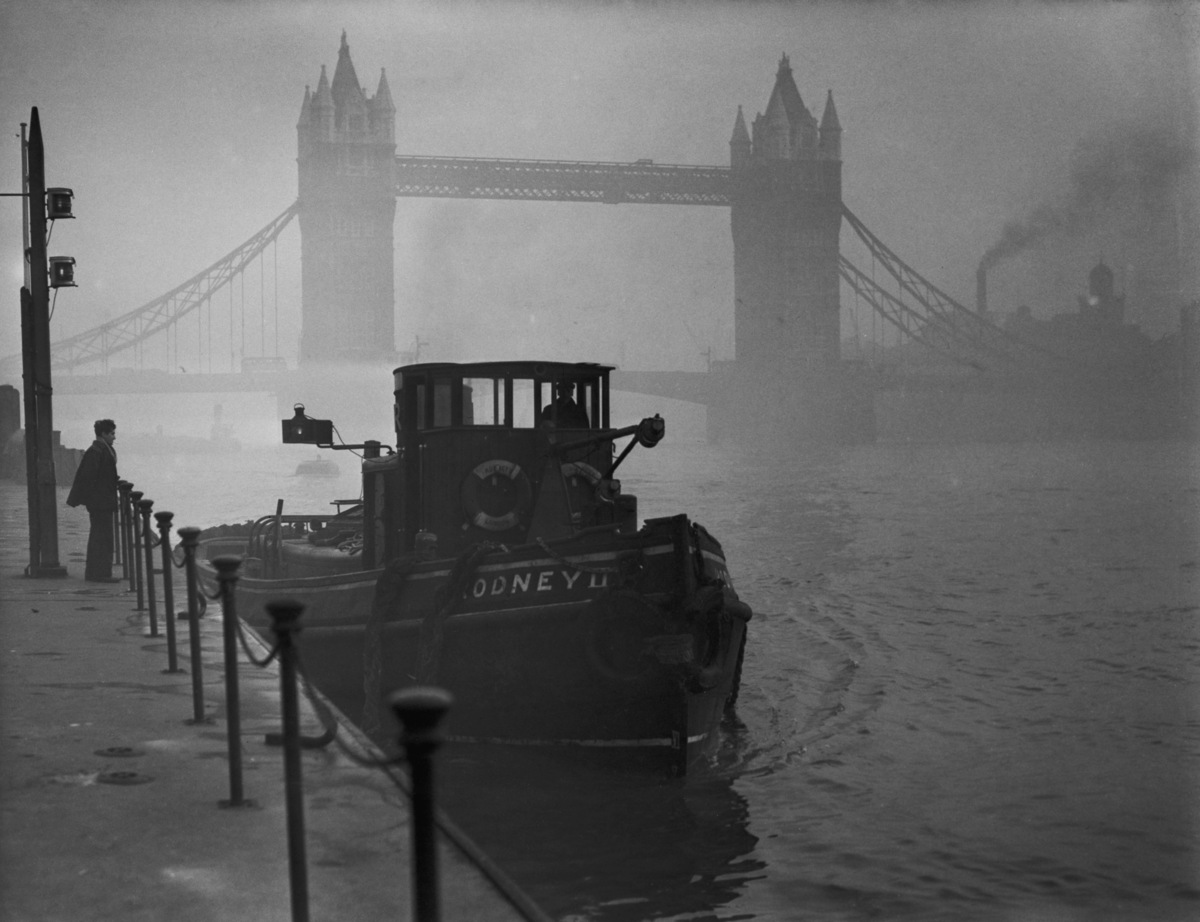
\includegraphics[scale=.8]{images/great_smog.jpg}
  \caption[Great smog of 1952]{Great smog of 1952 \cite{ElliotWagland2013}}
  \label{fig:interaction_design}
\end{figure}

The adverse health effects of pollution were noted in London's Great Smog of 1952. Thousands of people died in Greater London due to exposure over several days to a highly contaminated atmosphere. Many others became ill or experienced retarded symptoms \cite{Bell2008}. The fog originated from coal burning, vehicle exhaust and other atmospheric factors. Although many human activities which contribute to pollution have been brought in and change since, it has become evident the immediate and retarded health impact of pollution.

Pollution particles can be categorised into gaseous pollutants, persistent organic pollutants, heavy metals and particulate matter. They vary in their chemical composition, emission sources and impact on health. 

Gaseous pollutants are sulphur dioxide (\SOTWO), nitrogen oxides (\NOX), carbon monoxide (CO), ozone (\OTHREE) and volatile organic compounds (VOCs). The principal source of gaseous pollutants is the combustion of fossil fuels and diesel emission from vehicles. Nitrogen oxides (\NOX) is a general term that includes nitric oxide (NO) and nitrogen oxide \NOTWO. Gaseous pollutants can affect our health by inflaming the airways and lungs, and in the long term, affect the function of the lungs \cite{AirQualityExpertGroup2004} \cite{WHO2003}.

Particulate matter (PM) is a mixture of solid and liquid particles (such as sulphate, nitrates, ammonia, sodium chloride, black carbon, mineral dust and water). PM are categorised according to their diameter size measured in microns (\SI{}{\micro\metre}, one millionth of a metre). Particles smaller than 10 microns (\PMTEN) are known as coarse particles. Smaller particles with a size of up to 2.5 and 1 microns (\PMTWO and \PMONE) are known as fine and ultra-fine particles respectively. They are differentiated in sizes due to their aerodynamic properties, how they are transported into the air, as well as how far they can get into the respiratory system. According to the World Health Organisation, PM is the most harmful pollutant because it can pass through the nose and throat and enter the lungs. There is also evidence that it is associated with risk of cardiovascular disease \cite{Polichetti2009}. 

Air quality is also affected by pollution mixture in further complex chemical structures, temperature and humidity. \NOTWO, PM and O\textsubscript{3}  pollutants are transformed by atmospheric processes making it hard to evaluate their individual impact. As an example, ground level ozone is produced when sunlight interacts with \NOTWO and volatile organic compounds. Furthermore, \NOTWO and other nitrogen oxides also contribute to PM generation, making \NOX a particularly concerning pollutant.

\subsection{Air quality data dissemination}
The publication of air quality data aims to better inform and raise awareness amongst citizens who can then make more sustainable and environmental choices. According to Thinh and Vogel’s report for the Environmental Informatics and Systems Research journal, \quotes{what was lacking (and it still is), is a model for effective communicating of environmental information to the public} \cite{Thinh2007}. Terms like assessment, limit values, target values and concentration, among others, are commonly used by air quality data publishers to describe the current or forecasted quality status. However, there is not general agreement on how air quality information should be disseminated to the general public in a way that is understood immediately and intuitively by the wider public. 

In general, it is complex to categorise and establish measures for the different components of air pollution due their heterogeneous nature and the chemical reactions that occur between them. Measurement methods and units vary from institution to institution and regulation standards vary between countries, which may give rise to ambiguity. Furthermore, much of the available data is represented in a tabular format, including various information for individual pollutants, as exemplified in table \ref{tab:pollution_tabular_data}. This table was extracted from the  Department for Environment Food and Rural Affairs (DEFRA) website \cite{DepartmentforEnvironmenta}, and shows measures related to the air quality from a sensing station located in Deaconess Garden in the south of Edinburgh. At first glance the table poses key questions for the novice on air-quality trying to crack the data. Firstly, the pollution codes such as PM2.5, PM10, NO2, NOX as NO2 and their subtle differences must be understood. Secondly, some measurement units are tagged with the monitoring method used to extract the information, like the TEOM FDMS \footnote{Which indicates that the sensing methods were Tapered Element Oscillating Microbalance and Filter Dynamics Measurement System \cite{Quality2005}} tag. Lastly, it is difficult to know which measurements are of more interest given varying individual circumstances. As stated by Brimblecombe and Schuepbach \cite{P.Brimblecombe2008}, \quotes{many people complain that the information is unintelligible, while some have even seen it as an attempt of government to blind the public with science}.  All in all, understanding the meaning of the terms and values that are used to represent air quality data to the general public go beyond layman terms.
\begin{table}[ht]
\centering
\begin{adjustbox}{width=1.2\textwidth,center=\textwidth}
\begin{tabular}{rlrrrrrrr}
  \hline
 Pollutant & Date & Time & Measurement & Unit & Period & Comment  \\ \hline
    Ozone (O3) & 20/07/2016 & 07:00 & 63.06412 & µg/m3 & Hourly & - \\
    Nitric oxide (NO) & 20/07/2016 & 07:00 & 2.61933 & µg/m3 & Hourly & - \\
    Nitrogen dioxide (NO2) & 20/07/2016 & 07:00 & 27.34875 & µg/m3 & Hourly & - \\
    Nitrogen oxides as nitrogen dioxide (NOXasNO2) & 20/07/2016 & 07:00 & 31.36500 & µg/m3 & Hourly & - \\
	Sulphur dioxide (SO2) & 20/07/2016 & 07:00 & 14.63495 & µg/m3 & Hourly & - \\
	Carbon monoxide (CO) & 20/07/2016 & 07:00 & 0.081494 & mg/m3 & Hourly & - \\
	PM10 particulate matter (Hourly measured) (PM10) & 18/07/2016 & 15:00 & 10.900 & µg/m3 (TEOM FDMS) & Hourly & - No current data. \\
	Non-volatile PM10 (Hourly measured) (Non-volatile PM10) & 19/07/2016 & 07:00 & 26.700 & µg/m3 (TEOM FDMS) & Hourly & - No current data. \\
	Volatile PM10 (Hourly measured) (Volatile PM10) & 19/07/2016 & 07:00 & 5.500 & µg/m3 (TEOM FDMS) & Hourly & - No current data. \\
	PM2.5 particulate matter (Hourly measured) (PM2.5) & 18/07/2016 & 15:00 & 4.300 & µg/m3 (TEOM FDMS) & Hourly & - No current data. \\
	Non-volatile PM2.5 (Hourly measured) (Non-volatile PM2.5) & 19/07/2016 & 07:00 & 16.300 & µg/m3 (TEOM FDMS) & Hourly & - No current data. \\
	Volatile PM2.5 (Hourly measured) (Volatile PM2.5) & 19/07/2016 & 07:00 & 5.000 & µg/m3 (TEOM FDMS) & Hourly & - No current data. \\
	Modelled Wind Direction (Dir) & 19/07/2016 & 24:00 & 50.6 & \degree & Hourly & - No current data. \\
	Modelled Wind Speed (Speed) & 19/07/2016 & 24:00 & 6.2 & m/s & Hourly & - No current data. \\
	Modelled Temperature (Temp) & 19/07/2016 & 24:00 & 14.6 & °C & Hourly & - No current data. \\
	PM10 Ambient Temperature (AT10) & 19/07/2016 & 07:00 & 19.4 & °C & Hourly & - No current data. \\
	PM10 Ambient pressure measured (AP10) & 19/07/2016 & 07:00 & 989.0 & mb & Hourly & - No current data. \\
	PM2.5 Ambient Temperature (AT25 ) & 19/07/2016 & 07:00 & 17.5 & °C & Hourly & - No current data. \\
	PM2.5 Ambient Preasure (AP25) & 19/07/2016 & 07:00 & 988.0 & mb & Hourly & - No current data. \\
   \hline
\end{tabular}
\end{adjustbox}
\caption{Air quality tabular data representation. \cite{DepartmentforEnvironment}}
\label{tab:pollution_tabular_data}
\end{table} 

\subsection{The COMEAP air quality index and health advice}
In order to understand the correlation between air quality data and its effects on human health, the Committee on the Medical Effects of Air Pollutants (COMEAP) developed the air quality index based on health evidence. It is used to communicate real-time air quality levels and their short-term health effects for five selected harmful pollutants: particulate matter (\PMTEN and \PMTWO), ozone (\OTHREE), sulphur dioxide (\SOTWO), and nitrogen dioxide (\NOTWO) as shown in Figure \ref{fig:air_quality_index}. The index employs a colour scale and a number  to inform the concentrations of each specific pollutant. Four bands are employed: Low, Moderate, High and Very High. 

\begin{figure}[H]
\begin{adjustbox}{width=1\textwidth,center=\textwidth}
  \centering
  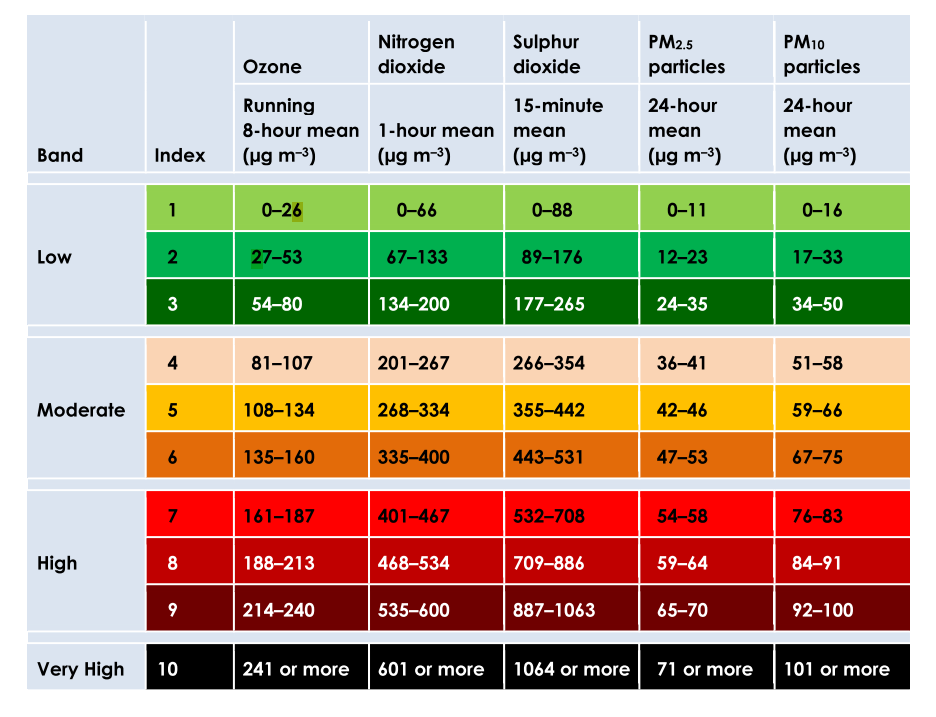
\includegraphics[scale=.8]{images/air_quality_index.png}
\end{adjustbox}
  \caption[The COMEAP air quality index]{The COMEAP air quality index \cite{HealthProtectionAgencyfortheCommitteeontheMedicalEffectsofAirPollutants2011}}
  \label{fig:air_quality_index}
\end{figure}

There is substantial evidence that the elderly, children, and people who suffer from chronic diseases such as asthma are in greater danger of suffering symptoms and health consequences from lower pollution concentrations than the general public \cite{Koenig1999} \cite{Kampa2008} \cite{Zones2010}. The COMEAP includes such population in their Air Quality Index to give such individuals the opportunity to modify their behaviour and reduce the severity of their symptoms. Furthermore, the air quality index is accompanied by health advice (Figure \ref{fig:air_quality_health_advice}) that provides specific health messages targeting both population groups, sensitive and non-sensitive providing information about the actions that should be taken to avoid symptoms and health effects.

\begin{figure}[H]
\begin{adjustbox}{width=1\textwidth,center=\textwidth}
  \centering
  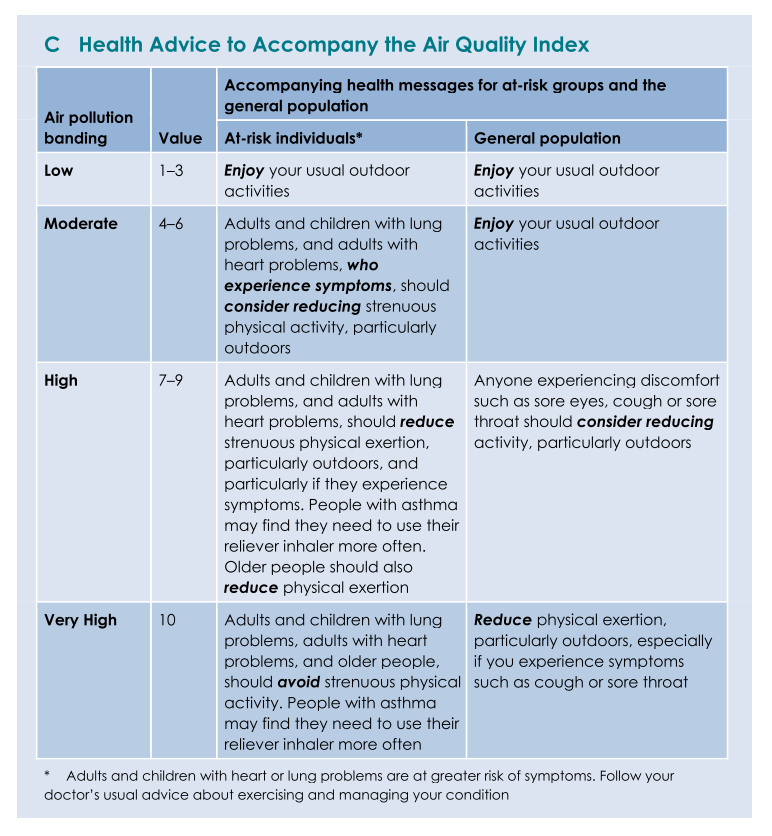
\includegraphics[scale=.8]{images/air_quality_health_advice.png}
\end{adjustbox}
  \caption[Air quality health advice]{Air quality health advice \cite{HealthProtectionAgencyfortheCommitteeontheMedicalEffectsofAirPollutants2011}}
  \label{fig:air_quality_health_advice}
\end{figure}


\subsection{Air quality sensors}

\begin{itemize}

\item Fixed sensors: 

Fixed sensors are installed and maintained by the UK government and local authorities in Scotland. There are of two kinds, automatic sensors from the Automatic Urban and Rural Network (AURN)\footnote{\url{https://uk-air.defra.gov.uk/networks/network-info?view=aurn}}, and non-automatic sensors maintained by Scottish local councils.

	\begin{itemize}
    
    \item Automatic sensors\footnote{\url{https://uk-air.defra.gov.uk/networks/network-info?view=non-automatic}} produce hourly concentrations and data is sent automatically over the network. Their purpose is to check that EU and other regulatory standards are being met as well as informing the public about air quality. These sensors monitor a wide range of pollutants (\NOX, \SOTWO, CO\textsubscript{2}, O\textsubscript{3}, \PMTWO and \PMTEN, as well as temperature and humidity) which are later collected and processed by Ricardo Energy and Environment\footnote{\url{http://ee.ricardo.com}} and presented on HTML webpages at the Scottish Air Quality website\footnote{\url{http://www.scottishairquality.co.uk/}}. Alternatively, CSV files provided on demand. The advantage of these sensors is its accuracy as well as the automatic workflow of the data. On the other hand, having few sensors spread around the city does not offer much resolution to current limitations. 
    \item Non-automatic sensors\footnote{\url{https://uk-air.defra.gov.uk/networks/network-info?view=non-automatic}} are commonly known as diffusion tubes. They offer higher resolution as there are over 100 situated in Edinburgh. The drawback is that samples must be collected physically, lessening the time at which the information can be communicated. Also, the data gathered is only limited to \NOTWO readings.
    \end{itemize}

\item Portable sensors: Their various advantages are that they can be carried throughout the day and allow for more personal and accurate readings based on the actual location of the user. The drawback is that some of them are limited to one pollutant, and the ones that can measure a range of different pollutants are still expensive. Examples are the Air Beam\footnote{\url{http://aircasting.org/}}, the Clean Space Tag\footnote{\url{https://store.clean.space/}} and the Libelium Gases PRO\footnote{\url{http://www.libelium.com/development/waspmote/documentation/gases-pro-board-technical-guide/}}. The first is open source and able to measure particle matter. The second is a proprietary project which only includes carbon monoxide readings and costs around 100\pounds. The latter measures a wider range of pollutants (CO, CO\textsubscript{2}, O\textsubscript{3}, \NOX and other gases) at a higher price (approximately \euro{}2000). 

\item Participatory sensors:

Some projects such as CitiSense \cite{Nikzad2012} include users as 'human sensors' by reading their perceptions towards air quality in certain locations. This method aims to get more fine-grained information about air quality and engage the citizens in the pollution problem a possible solution. 

\end{itemize}



